\begin{center}
\Huge
Fordoblingskonstanten for eksponentialfunktioner
\end{center}
\section*{Fordoblingskonstanten}
\stepcounter{section}
Perspektivet var før at overveje, hvordan funktionsværdien af eksponentiel vækst udvikler sig, når vi øger $x$ med $1$. Vi kan tilsvarende betragte problemet fra den modsatte side: hvad skal vi øge $x$ med for at fordoble/halvere funktionsværdien. Vi skal altså bestemme en størrelse $T_2$, så 
\begin{align*}
f(x+T_2) = 2f(x)
\end{align*}
for en eksponentialfunktion $f$. Denne idé er præsenteret i Figur \ref{fig:Fordobling}. 
\begin{figure}[H]
\center
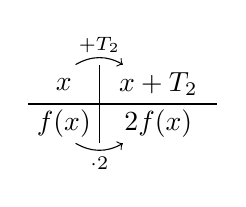
\begin{tikzpicture}
\foreach \i in {0}{
\draw (\i*0.9,0) -- (\i*0.9,1);
}
\draw (-0.9,0.5) -- (1.5,0.5);
\foreach \i in {0}{
\node at (\i*0.9+ 0.75,0.75) {$x+T_2$};
\node at (\i*0.9+0.75,0.25) {$2f(x)$};
}
\node at (-0.45,0.75) {$x$};
\node at (-0.45,0.25) {$f(x)$};
\foreach \i in {0}{
\draw [->] (\i*0.9-0.3,1) to [out=30,in=150] (\i*0.9+0.3,1);
\node at (\i*0.9,1.25) {$\scriptstyle+T_2$};
\draw [->] (\i*0.9-0.3,-0) to [out=-30,in=-150] (\i*0.9+0.3,-0);
\node at (\i*0.9,-0.25) {$\scriptstyle\cdot 2$};
}
\end{tikzpicture}

\caption{Fordoblingskonstant}
\label{fig:Fordobling}
\end{figure}

Dette kan tilsvarende ses grafisk på Figur \ref{fig:grafisk}
\begin{figure}[H]
	\centering
	\begin{tikzpicture}
		\begin{axis}
		[axis lines = center,
		ticks = none,
		xmin = -1, xmax = 4,
		ymin = -2,
		ylabel = $y$, xlabel = $x$
		]
			\addplot[thick, color = olive, samples = 100] {2^x};
			\draw[dashed, thick, color = teal] (axis cs: 1,0) to (axis cs: 1,2);
			\draw[dashed, thick, color = teal] (axis cs: 2,0) to (axis cs: 2,4);
			\draw[dashed, thick, color = teal] (axis cs: 0,2) to (axis cs: 1,2);
			\draw[dashed, thick, color = teal] (axis cs: 0,4) to (axis cs: 2,4);
			\node at (axis cs:-0.4,2) {$f(x_0)$};
			\node at (axis cs:-0.45,4) {$2f(x_0)$};
			\node at (axis cs: 1,-1) {$x_0$};
			\node at (axis cs: 2,-1) {$x_0 + T_2$};
		\end{axis}
	\end{tikzpicture}
	\caption{Grafisk præsentation af fordoblingskonstanten.}
	\label{fig:grafisk}
\end{figure}


\begin{exa}
	Vi betragter eksponentialfunktionen $f$ givet ved
	\begin{align*}
		f(x) = 2^x.
	\end{align*}
	Grafen for denne kan ses på Figur \ref{fig:eksempel}.
	\begin{figure}[H]
		\centering
		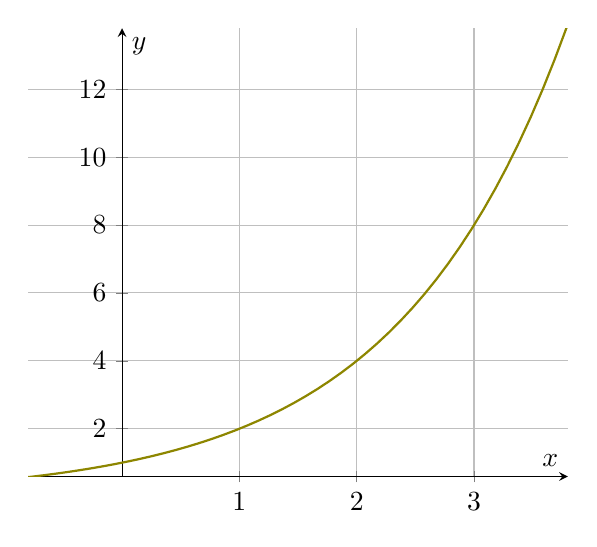
\begin{tikzpicture}
			\begin{axis}[axis lines = center, grid = both,
			xmin = -0.8, xmax = 3.8,
			xlabel = $x$,ylabel = $y$
			]
				\addplot[thick, color = olive, samples = 100] {2^x};
			\end{axis}
		\end{tikzpicture}
		\caption{Graf for funktionen $f(x) = 2^x$.}
		\label{fig:eksempel}
	\end{figure}
	Vi kan på figuren aflæse, at fordoblingskonstanten for $f$ er $1$, da vi skal øge $x$ med $1$ for at funktionsværdien fordobles. 
\end{exa}
For eksponentialvækst, hvor fremskrivningsfaktoren $a$ er større end $1$ er det muligt at finde et sådan tal $T_2>0$. Følgende sætning fortæller, hvordan vi skal finde dette tal, og vi kalder tallet for \textit{Fordoblingskonstanten for f}.
\begin{setn}
For en eksponentialfunktion $f$ gælder det, at fordoblingskonstanten $T_2$, der opfylder, at
\begin{align*}
f(x+T_2) = 2f(x)
\end{align*}
er givet ved 
\begin{align*}
T_2 = \frac{\log(2)}{\log(a)} = \frac{\ln(2)}{\ln(a)}
\end{align*}
Tilsvarende er halveringskonstanten $T_{1/2}$, der opfylder, at 
\begin{align*}
f(x+T_{1/2}) = \frac{1}{2}f(x)
\end{align*}
bestemt ved
\begin{align*}
T_{1/2} = \frac{\ln(1/2)}{\ln(a)} = \frac{\log(1/2)}{\log(a)}.
\end{align*}
Desuden gælder der, at $a = \sqrt[T_2]{2}= \sqrt[T_{1/2}]{1/2}$
\end{setn}
\begin{proof}
Vi beviser tilfældet for fordoblingskonstanten. Tilfældet for halveringskonstanten beviset fuldstændig analogt. Lad os derfor for en eksponentialfunktion $f$ givet ved
\begin{align*}
f(x) = b\cdot a^x
\end{align*}
antage, at tallet $T_2$ opfylder, at $f(x+T_2) = 2f(x)$ for alle $x\in \mathbb{R}$. Vi har så, at 
\begin{align*}
f(x+T_2) = 2f(x) \ &\Leftrightarrow \ b\cdot a^{x}a^{T_2}=2b\cdot a^x\\
&\Leftrightarrow\ a^{T_2} = 2\\
&\Leftrightarrow\ \ln(a^{T_2}) = \ln(2)\\
&\Leftrightarrow\ T_2\ln(a) = \ln(2)\\
&\Leftrightarrow\ T_2 = \frac{\ln(2)}{\ln(a)},
\end{align*}
og vi har givet et bevis for fordoblingskonstanten. Siden vi har, at $a^{T_2} = 2$, så må der desuden gælde, at $a=\sqrt[T_2]{2}$, da $a>0$. 
\end{proof}

\begin{exa}
	Vi bruger sætningen til at bestemme fordoblingskonstanten for eksponentialfunktionen
	\begin{align*}
		f(x) = 2^x.
	\end{align*}
	Vi får, at 
	\begin{align*}
		T_2 = \frac{\ln(2)}{\ln(a)} = \frac{\ln(2)}{\ln(2)} = 1,
	\end{align*}
	som også var det vi kom frem til ved at bruge Figur \ref{fig:eksempel}.
\end{exa}

\newpage
\subsection*{Opgave 1}
Aflæs fordoblings/halveringskonstanten for følgende eksponentialfunktioner.
\begin{center}
\resizebox{0.45\textwidth}{!}{
	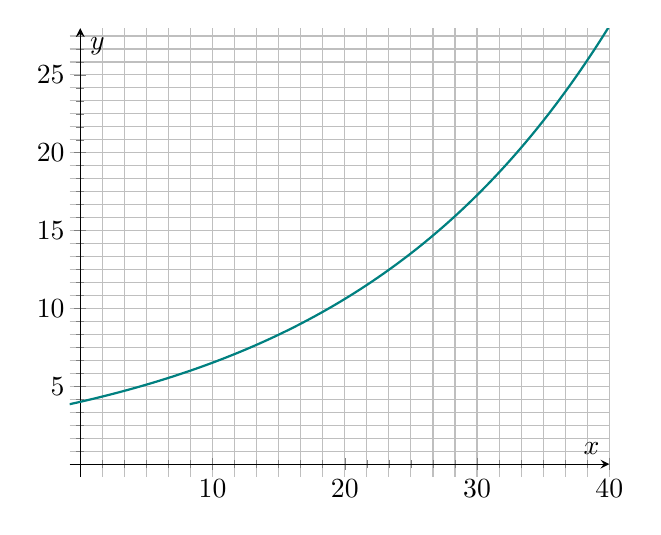
\begin{tikzpicture}
		\begin{axis}[
		axis lines = center,
		xmin = -0.8, xmax = 40,
		ymin = -0.8,ymax = 28,
		grid = both,
		minor tick num = 5,
		xlabel = $x$, ylabel = $y$,
		]
			\addplot[thick, samples = 1000, color = teal, domain = -0.8:40] {4*1.05^x};
		\end{axis}
	\end{tikzpicture}	
}	
\resizebox{0.45\textwidth}{!}{
	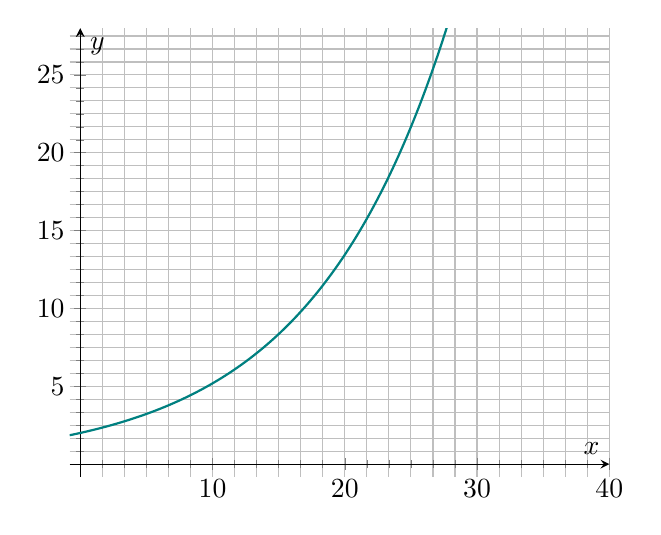
\begin{tikzpicture}
		\begin{axis}[
		axis lines = center,
		xmin = -0.8, xmax = 40,
		ymin = -0.8,ymax = 28,
		grid = both,
		minor tick num = 5,
		xlabel = $x$, ylabel = $y$
		]
			\addplot[thick, samples = 1000, color = teal, domain = -0.8:40] {2*1.1^x};
		\end{axis}
	\end{tikzpicture}
}
\resizebox{0.45\textwidth}{!}{
	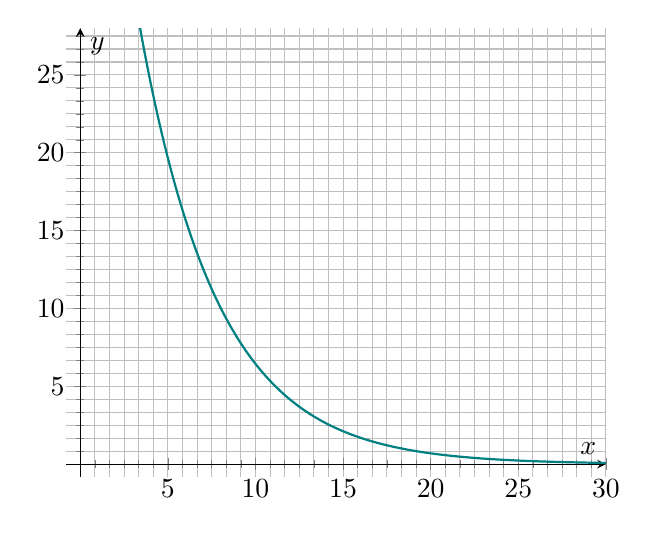
\begin{tikzpicture}
		\begin{axis}[
		axis lines = center,
		xmin = -0.8, xmax = 30,
		ymin = -0.8,ymax = 28,
		grid = both,
		minor tick num = 5,
		xlabel = $x$, ylabel = $y$
		]
			\addplot[thick, samples = 1000, color = teal, domain = -0.8:40] {60*0.8^x};
		\end{axis}
	\end{tikzpicture}
}
\resizebox{0.45\textwidth}{!}{
	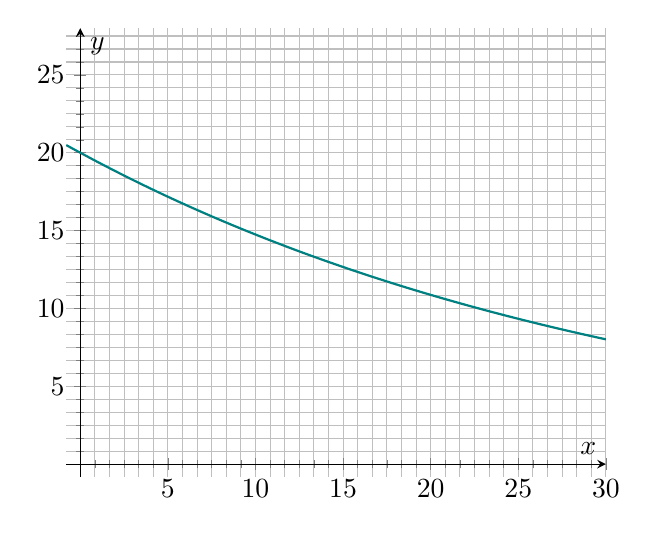
\begin{tikzpicture}
		\begin{axis}[
		axis lines = center,
		xmin = -0.8, xmax = 30,
		ymin = -0.8,ymax = 28,
		grid = both,
		minor tick num = 5,
		xlabel = $x$, ylabel = $y$
		]
			\addplot[thick, samples = 1000, color = teal, domain = -0.8:40] {20*0.97^x};
		\end{axis}
	\end{tikzpicture}
}
\end{center}

\subsection*{Opgave 2}
Bestem fordoblingskonstanten eller halveringskonstanten for følgende eksponentialfunktioner
\begin{align*}
	&1) \ 5\cdot 2^x   &&2) \ 7\cdot 0.95^x   \\
	&3) \ 1.03\cdot 1.004^x   &&4) \ 6\cdot 5.09^x   \\
	&5) \ 0.01\cdot 1.75^x   &&6) \ 7.19\cdot 1.179^x   \\		
	&7) \ 10\cdot 0.1^x   && 7) \ 6.13 \cdot 10^x  
\end{align*}


\subsection*{Opgave 3}
Bestem enten fordoblings eller halveringskonstanten for følgende eksponentialfunktioner
\begin{align*}
&1) \ f_1(x) = 0.5\cdot 2^x   &&2) \ f_2(x)=2\cdot 0.5^x  \\
&3) \ f_3(x) = 2000\cdot(0.003)^x  &&4) \ f_4(x) = 4\e^x  \\
\end{align*}

\subsection*{Opgave 4}

\begin{enumerate}[label=\roman*)]
	\item En bakteriekoloni vokser med 30 procent per døgn. Bestem fordoblingskonstanten for denne bakteriekoloni.
	\item En radioaktiv isotop henfalder med 10 procent om året. Bestem halveringskonstanten for denne isotop.
	\item Befolkningen i en by vokser med 2 procent om året. Bestem fordoblingskonstanten for befolkningen. 
	\item Du får 4 procent på en højrentekonto i banken. Hvor længe vil der gå, før du har fordoblet dine penge?
	\item Infektionstallet for en person falder med 12 procent i timen. Hvad er halveringskonstanten for infektionstallet?
\end{enumerate}
\newpage
\subsection*{Opgave 5}
Tetrahydrocannabinol (THC) er det primære psykoaktive stof i hampplanten. Koncentrationen af stoffet efter indtagelse hos en bestemt person kan ses af Tabel \ref{tab:cannabis}.

\begin{table}[H]
	\centering
	\rowcolors{2}{gray!25}{white}
	\begin{tabular}{cc}
		\textbf{Tid i timer} & \textbf{Koncentration i mg/L} \\

		0 & 0.30249 \\

		8 & 0.24512 \\
 
		16 &  0.20132 \\

		24 & 0.16371 \\

		32 & 0.13303\\

		40 & 0.11069\\

		48 & 0.08757\\
		56 & 0.07317\\

		64 & 0.05748
	\end{tabular}
	\caption{Koncentration af tetrahydrocannabiol (THC)}
	\label{tab:cannabis}
\end{table}

Det antages at sammenhængen mellem antal forløbne timer $x$ og blodkoncentrationen af THC $f(x)$ er givet ved en sammenhæng af typen
\begin{align*}
	f(x) = b \cdot a^x
\end{align*}
\begin{enumerate}[label=\roman*)]
	\item Lav regression på observationerne fra Tabel \ref{tab:cannabis} og bestem en forskrift for $f$.
	\item Bestem halveringskonstanten for $f$.
\end{enumerate}
Et stof eller lægemiddel vil betragtes som helt metaboliseret efter fem halveringstider.

\begin{enumerate}[label=\roman*)]
	\setcounter{enumi}{2}
	\item Hvor lang tid skal der gå, før vi kan sige, at der ikke er mere THC i kroppen på personen?
\end{enumerate}
